\documentclass[11pt,a4paper]{report}
\usepackage[textwidth=37em,vmargin=30mm]{geometry}
\usepackage{calc,xunicode,amsmath,amssymb,paralist,enumitem,tabu,booktabs,datetime2,xeCJK,xeCJKfntef,listings}
\usepackage{tocloft,fancyhdr,tcolorbox,xcolor,graphicx,eso-pic,xltxtra,xelatexemoji}

\newcommand{\envyear}[0]{2025}
\newcommand{\envdatestr}[0]{2025-09-08}
\newcommand{\envfinaldir}[0]{webdb/2025/20250908/final}

\usepackage[hidelinks]{hyperref}
\hypersetup{
    colorlinks=false,
    pdfpagemode=FullScreen,
    pdftitle={Web Digest - \envdatestr}
}

\setlength{\cftbeforechapskip}{10pt}
\renewcommand{\cftchapfont}{\rmfamily\bfseries\large\raggedright}
\setlength{\cftbeforesecskip}{2pt}
\renewcommand{\cftsecfont}{\sffamily\small\raggedright}

\setdefaultleftmargin{2em}{2em}{1em}{1em}{1em}{1em}

\usepackage{xeCJK,xeCJKfntef}
\xeCJKsetup{PunctStyle=plain,RubberPunctSkip=false,CJKglue=\strut\hskip 0pt plus 0.1em minus 0.05em,CJKecglue=\strut\hskip 0.22em plus 0.2em}
\XeTeXlinebreaklocale "zh"
\XeTeXlinebreakskip = 0pt


\setmainfont{Brygada 1918}
\setromanfont{Brygada 1918}
\setsansfont{IBM Plex Sans}
\setmonofont{JetBrains Mono NL}
\setCJKmainfont{Noto Serif CJK SC}
\setCJKromanfont{Noto Serif CJK SC}
\setCJKsansfont{Noto Sans CJK SC}
\setCJKmonofont{Noto Sans CJK SC}

\setlength{\parindent}{0pt}
\setlength{\parskip}{8pt}
\linespread{1.15}

\lstset{
	basicstyle=\ttfamily\footnotesize,
	numbersep=5pt,
	backgroundcolor=\color{black!5},
	showspaces=false,
	showstringspaces=false,
	showtabs=false,
	tabsize=2,
	captionpos=b,
	breaklines=true,
	breakatwhitespace=true,
	breakautoindent=true,
	linewidth=\textwidth
}






\newcommand{\coverpic}[2]{
    % argv: itemurl, authorname
    Cover photo by #2~~(\href{#1}{#1})
}
\newcommand{\makeheader}[0]{
    \begin{titlepage}
        % \newgeometry{hmargin=15mm,tmargin=21mm,bmargin=12mm}
        \begin{center}
            
            \rmfamily\scshape
            \fontspec{BaskervilleF}
            \fontspec{Old Standard}
            \fontsize{59pt}{70pt}\selectfont
            WEB\hfill DIGEST
            
            \vfill
            % \vskip 30pt
            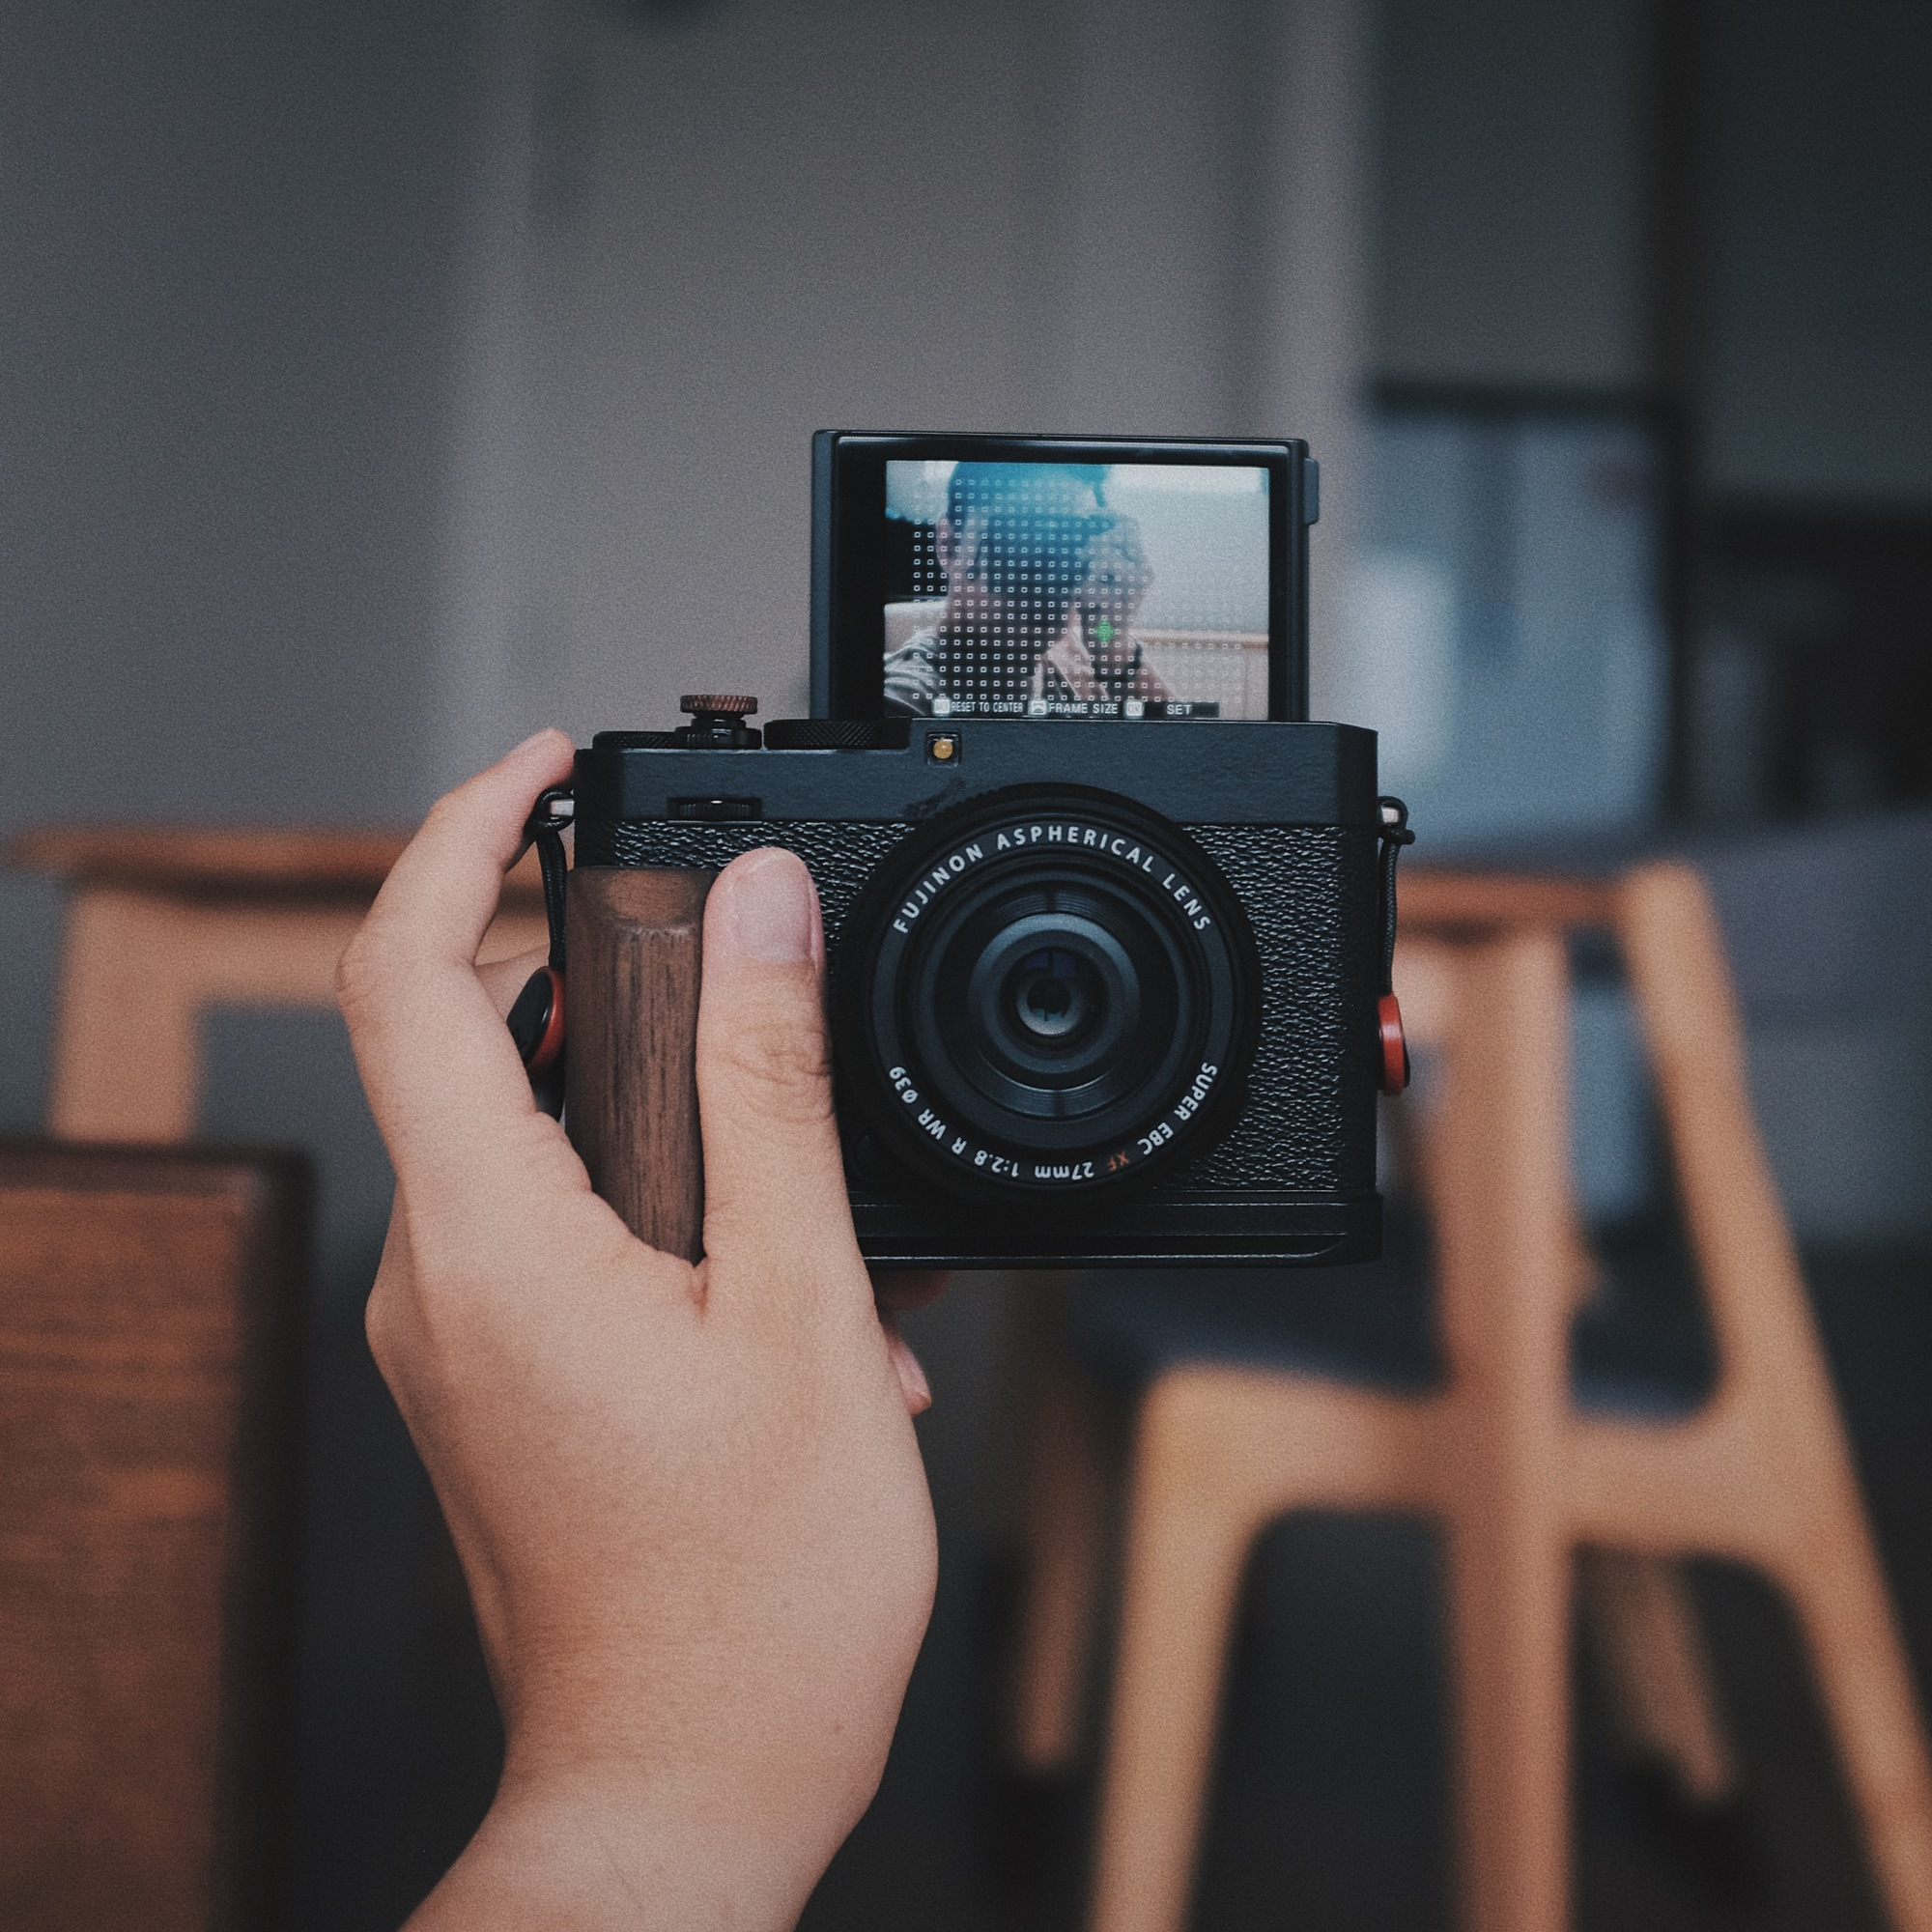
\includegraphics[width=\linewidth]{\envfinaldir/coverpic-prod.jpg}\par
            % \vskip 30pt
            \vfill

            \normalsize\rmfamily\scshape
            \copyright{} The Web Digest Project \hfill\large \envdatestr
        \end{center}
    \end{titlepage}
    % \restoregeometry
}
\newcommand{\simplehref}[1]{%
    \textcolor{blue!80!green}{\href{#1}{#1}}%
}
\renewcommand{\contentsname}{\center\Huge\sffamily\bfseries Contents\par\vskip 20pt}
\newcounter{ipartcounter}
\setcounter{ipartcounter}{0}
\newcommand{\ipart}[1]{
    % \vskip 20pt
    \clearpage
    \stepcounter{ipartcounter}
    \phantomsection
    \addcontentsline{toc}{chapter}{#1}
    % \begin{center}
    %     \Huge
    %     \sffamily\bfseries
    %     #1
    % \end{center}
    % \vskip 20pt plus 7pt
}
\newcounter{ichaptercounter}
\setcounter{ichaptercounter}{0}
\newcommand{\ichapter}[1]{
    % \vskip 20pt
    \clearpage
    \stepcounter{ichaptercounter}
    \phantomsection
    \addcontentsline{toc}{section}{\numberline{\arabic{ichaptercounter}}#1}
    \begin{center}
        \Huge
        \sffamily\bfseries
        #1
    \end{center}
    \vskip 20pt plus 7pt
}
\newcommand{\entrytitlefont}[1]{\subsection*{\raggedright\Large\sffamily\bfseries#1}}
\newcommand{\entryitemGeneric}[2]{
    % argv: title, url
    \parbox{\linewidth}{
        \entrytitlefont{#1}\par\vskip 5pt
        \footnotesize\ttfamily\mdseries
        \simplehref{#2}
    }\vskip 11pt plus 11pt minus 1pt
}
\newcommand{\entryitemGithub}[3]{
    % argv: title, url, desc
    \parbox{\linewidth}{
        \entrytitlefont{#1}\par\vskip 5pt
        \footnotesize\ttfamily\mdseries
        \simplehref{#2}\par\vskip 5pt
        \small\rmfamily\mdseries#3
    }\vskip 11pt plus 11pt minus 1pt
}
\newcommand{\entryitemAp}[3]{
    % argv: title, url, desc
    \parbox{\linewidth}{
        \entrytitlefont{#1}\par\vskip 5pt
        \footnotesize\ttfamily\mdseries
        \simplehref{#2}\par\vskip 5pt
        \small\rmfamily\mdseries#3
    }\vskip 11pt plus 11pt minus 1pt
}
\newcommand{\entryitemHackernews}[3]{
    % argv: title, hnurl, rawurl
    % \parbox{\linewidth}{
    %     \entrytitlefont{#1}\par\vskip 5pt
    %     \footnotesize\ttfamily\mdseries
    %     \simplehref{#3}\par
    %     \textcolor{black!50}{\href{#2}{#2}}
    % }\vskip 11pt plus 11pt minus 1pt
    \begin{minipage}{\linewidth}
            \entrytitlefont{#1}\par\vskip 5pt
            \footnotesize\ttfamily\mdseries
            \simplehref{#3}\par
            \textcolor{black!50}{\href{#2}{#2}}
    \end{minipage}\par\vskip 11pt plus 11pt minus 1pt
}







\begin{document}

\makeheader

\tableofcontents\clearpage




\ipart{Developers}
\ichapter{Hacker News}
\entryitemTwoLinks{Pico CSS – Minimal CSS Framework for Semantic HTML}{https://news.ycombinator.com/item?id=45161855}{https://picocss.com}

\entryitemTwoLinks{Everything from 1991 Radio Shack ad I now do with my phone (2014)}{https://news.ycombinator.com/item?id=45161816}{https://www.trendingbuffalo.com/life/uncle-steves-buffalo/everything-from-1991-radio-shack-ad-now/}

\entryitemTwoLinks{Keeping secrets out of logs (2024)}{https://news.ycombinator.com/item?id=45160774}{https://allan.reyes.sh/posts/keeping-secrets-out-of-logs/}

\entryitemTwoLinks{The MacBook has a sensor that knows the exact angle of the screen hinge}{https://news.ycombinator.com/item?id=45158968}{https://twitter.com/samhenrigold/status/1964428927159382261}

\entryitemTwoLinks{Nepal Bans 26 Social Media Platforms, Including Facebook and YouTube}{https://news.ycombinator.com/item?id=45158877}{https://www.nytimes.com/2025/09/07/world/asia/nepal-bans-social-media-platforms.html}

\entryitemTwoLinks{Delayed Security Patches for AOSP (Android Open Source Project)}{https://news.ycombinator.com/item?id=45158523}{https://twitter.com/grapheneos/status/1964561043906048183}

\entryitemTwoLinks{Belling the Cat}{https://news.ycombinator.com/item?id=45157906}{https://en.wikipedia.org/wiki/Belling\_the\_Cat}

\entryitemTwoLinks{Air pollution directly linked to increased dementia risk}{https://news.ycombinator.com/item?id=45157897}{https://www.nature.com/articles/d41586-025-02844-9}

\entryitemTwoLinks{Postal traffic to US down by over 80\% amid tariffs, UN says}{https://news.ycombinator.com/item?id=45157837}{https://www.dw.com/en/postal-traffic-to-us-down-by-over-80-amid-tariffs-un-says/a-73905988}

\entryitemTwoLinks{More and more people are tuning the news out: 'Now I don't have that anxiety}{https://news.ycombinator.com/item?id=45157784}{https://www.theguardian.com/society/ng-interactive/2025/sep/01/news-avoidance-high-anxiety}

\entryitemTwoLinks{Show HN: Semantic grep with local embeddings}{https://news.ycombinator.com/item?id=45157223}{https://github.com/BeaconBay/ck}

\entryitemTwoLinks{Serverless Horrors}{https://news.ycombinator.com/item?id=45157110}{https://serverlesshorrors.com/}

\entryitemTwoLinks{Show HN: I'm a dermatologist and I vibe coded a skin cancer learning app}{https://news.ycombinator.com/item?id=45157020}{https://molecheck.info/}

\entryitemTwoLinks{What is the origin of the private network address 192.168.*.*? (2009)}{https://news.ycombinator.com/item?id=45156826}{https://lists.ding.net/othersite/isoc-internet-history/2009/oct/msg00000.html}

\entryitemTwoLinks{I am giving up on Intel and have bought an AMD Ryzen 9950X3D}{https://news.ycombinator.com/item?id=45155986}{https://michael.stapelberg.ch/posts/2025-09-07-bye-intel-hi-amd-9950x3d/}

\entryitemTwoLinks{The ``impossibly small'' Microdot web framework}{https://news.ycombinator.com/item?id=45155682}{https://lwn.net/Articles/1034121/}

\entryitemTwoLinks{Unofficial Windows 11 requirements bypass tool allows disabling all AI features}{https://news.ycombinator.com/item?id=45155398}{https://www.neowin.net/news/unofficial-windows-11-requirements-bypass-tool-now-allows-you-to-disable-all-ai-features/}

\entryitemTwoLinks{The Claude Code Framework Wars}{https://news.ycombinator.com/item?id=45155302}{https://shmck.substack.com/p/claude-code-framework-wars}

\entryitemTwoLinks{RFC 3339 vs. ISO 8601}{https://news.ycombinator.com/item?id=45155179}{https://ijmacd.github.io/rfc3339-iso8601/}

\entryitemTwoLinks{Show HN: Lightweight tool for managing Linux virtual machines}{https://news.ycombinator.com/item?id=45154857}{https://github.com/ccheshirecat/flint}\ichapter{Phoronix}
\entryitemGeneric{\hskip 0pt{}Linux 6.17-rc5 Released With NVIDIA "Nouveau" Driver Stability Issues Addressed}{https://www.phoronix.com/news/Linux-6.17-rc5}

\entryitemGeneric{\hskip 0pt{}Intel Preps Wildcat Lake Display Support For Linux 6.18, "enable\_panel\_replay" Option}{https://www.phoronix.com/news/Intel-DRM-Next-Linux-6.18}

\entryitemGeneric{\hskip 0pt{}Hangover 10.14 Released With Updated FEX, Box64 \& DXVK}{https://www.phoronix.com/news/Hangover-10.14}

\entryitemGeneric{\hskip 0pt{}Imagination PowerVR Driver With Linux 6.18 To Support RISC-V}{https://www.phoronix.com/news/Linux-6.18-PowerVR-RISC-V}

\entryitemGeneric{\hskip 0pt{}FreeBSD 15.0 Alpha 1 Released For Early Testing}{https://www.phoronix.com/news/FreeBSD-15.0-Alpha-1}

\entryitemGeneric{\hskip 0pt{}Ubuntu 25.10 Enters Its UI Freeze}{https://www.phoronix.com/news/Ubuntu-25.10-UI-Freeze}

\entryitemGeneric{\hskip 0pt{}Intel PEPC 1.6 Released For Tuning Efficiency Latency Control "ELC" With Xeon 6 CPUs}{https://www.phoronix.com/news/Intel-PEPC-1.6}

\entryitemGeneric{\hskip 0pt{}Linux 6.17 Lands Fixes For Upcoming Rust 1.91}{https://www.phoronix.com/news/Linux-6.17-Rust-1.91}

\entryitemGeneric{\hskip 0pt{}Debian 13.1 Released With An Initial Batch Of Fixes}{https://www.phoronix.com/news/Debian-13.1-Released}


\ipart{Developers~~~~(zh-Hans)}
\ichapter{Solidot}
\entryitemGeneric{\hskip 0pt{}特斯拉改变了 Full Self-Driving 的意义,放弃承诺自动驾驶}{https://www.solidot.org/story?sid=82243}

\entryitemGeneric{\hskip 0pt{}美国计划限制进口中国无人机}{https://www.solidot.org/story?sid=82242}

\entryitemGeneric{\hskip 0pt{}Anthropic 向图书作者支付 15 亿美元和解侵权诉讼}{https://www.solidot.org/story?sid=82241}

\entryitemGeneric{\hskip 0pt{}Firefox 将于 2026 年 9 月停止支持 32 位 Linux 系统}{https://www.solidot.org/story?sid=82240}

\entryitemGeneric{\hskip 0pt{}Google 因广告技术业务的反垄断行为被欧盟罚款 34.5 亿美元 }{https://www.solidot.org/story?sid=82239}

\entryitemGeneric{\hskip 0pt{}英国政府试用 M365 Copilot 后未发现明显的生产力提升}{https://www.solidot.org/story?sid=82238}

\entryitemGeneric{\hskip 0pt{}阿富汗地震已造成逾 3000 人死亡}{https://www.solidot.org/story?sid=82237}

\entryitemGeneric{\hskip 0pt{}Mark Zuckerberg 起诉 Mark Zuckerberg}{https://www.solidot.org/story?sid=82236}

\entryitemGeneric{\hskip 0pt{}上厕所时用智能手机大幅增加痔疮风险}{https://www.solidot.org/story?sid=82235}

\entryitemGeneric{\hskip 0pt{}人工甜味剂与认知能力下降相关,相当于衰老 1.6 年}{https://www.solidot.org/story?sid=82234}

\entryitemGeneric{\hskip 0pt{}Anthropic 禁止中国控股公司使用 Claude}{https://www.solidot.org/story?sid=82233}

\entryitemGeneric{\hskip 0pt{}尼泊尔屏蔽大部分社媒平台}{https://www.solidot.org/story?sid=82232}

\entryitemGeneric{\hskip 0pt{}微软开源 6502 BASIC }{https://www.solidot.org/story?sid=82231}

\entryitemGeneric{\hskip 0pt{}英特尔研发支出超英伟达和 AMD}{https://www.solidot.org/story?sid=82230}

\entryitemGeneric{\hskip 0pt{}Atlassian 以 6.1 亿美元收购 Browser Company  }{https://www.solidot.org/story?sid=82229}

\entryitemGeneric{\hskip 0pt{}美国失业人数超过招聘人数}{https://www.solidot.org/story?sid=82228}\ichapter{V2EX}
\entryitemGeneric{\hskip 0pt{}[分享创造] 整理了一个 AI 提示词库}{https://www.v2ex.com/t/1157671}

\entryitemGeneric{\hskip 0pt{}[分享创造] 27 天,达成第一个 1000⭐️ 开源项目,回来感谢}{https://www.v2ex.com/t/1157670}

\entryitemGeneric{\hskip 0pt{}[程序员] 尝试了 Copilot, Windsurf, Kiro, Trae 国际, Cursor,仅就编辑协作来说, Cursor 还是第一}{https://www.v2ex.com/t/1157669}

\entryitemGeneric{\hskip 0pt{}[MacBook Pro] 小黄鱼上的 m3max128g8t16 寸可靠嘛?}{https://www.v2ex.com/t/1157668}

\entryitemGeneric{\hskip 0pt{}[问与答] 有在看月全食的朋友吗}{https://www.v2ex.com/t/1157666}

\entryitemGeneric{\hskip 0pt{}[Apple] M3 Ultra or M4 Max 能正常服役接下来 10 年么}{https://www.v2ex.com/t/1157665}

\entryitemGeneric{\hskip 0pt{}[职场话题] 95 年 30 岁,一般的 211 本硕,本科消防,硕士安全,想转 iT 赴日,老哥们有没有建议或者意见}{https://www.v2ex.com/t/1157664}

\entryitemGeneric{\hskip 0pt{}[问与答] 公网上的 windows 11 如何完成迁移?}{https://www.v2ex.com/t/1157663}

\entryitemGeneric{\hskip 0pt{}[NAS] 截止发帖时,最好的 6 盘位以上 NAS 系统方案是不是 Unraid 底层+飞牛应用层?}{https://www.v2ex.com/t/1157662}

\entryitemGeneric{\hskip 0pt{}[Apple] 国行 iphone16pro 有必要换成 日版吗?}{https://www.v2ex.com/t/1157661}

\entryitemGeneric{\hskip 0pt{}[酷工作] 招聘: 法币出入金 产品经理 跨境电商技术负责人 资深后端开发-链上 北美区域负责人 RWA 产品经理, 后端工程师(DeFi), Golang \& Flutter \& C++交易系统 高级运维总监, 资深\&首席架构师}{https://www.v2ex.com/t/1157660}

\entryitemGeneric{\hskip 0pt{}[问与答] 最近抖音上刷到很多程序员博主都在介绍远程工作的}{https://www.v2ex.com/t/1157659}

\entryitemGeneric{\hskip 0pt{}[问与答] 问大家一个问题,学区房真的非买不可吗?}{https://www.v2ex.com/t/1157658}

\entryitemGeneric{\hskip 0pt{}[分享发现] 电脑上的微信是不是监控你的操作?}{https://www.v2ex.com/t/1157655}

\entryitemGeneric{\hskip 0pt{}[程序员] 缓存击穿(Cache Breakdown)是不是一个很迷惑的翻译}{https://www.v2ex.com/t/1157654}

\entryitemGeneric{\hskip 0pt{}[生活] 我有一个朋友,经历了一段很不美好的感情,发出来,记录一下吧}{https://www.v2ex.com/t/1157653}

\entryitemGeneric{\hskip 0pt{}[问与答] 求教如何让家中宽带对外提供服务,但不被运营商发现}{https://www.v2ex.com/t/1157652}

\entryitemGeneric{\hskip 0pt{}[职场话题] 好奇问问,有没有摸鱼被公司开除的}{https://www.v2ex.com/t/1157651}

\entryitemGeneric{\hskip 0pt{}[iPhone] 网易客户端的首页刷新是走了什么协议吗}{https://www.v2ex.com/t/1157648}

\entryitemGeneric{\hskip 0pt{}[宽带症候群] 上海移动 2000M 体验}{https://www.v2ex.com/t/1157647}

\entryitemGeneric{\hskip 0pt{}[问与答] 求教大佬们使用 zerotier 组网后,如何让 A 服务可以访问 B 服务,B 服务不能主动访问 A 服务}{https://www.v2ex.com/t/1157646}

\entryitemGeneric{\hskip 0pt{}[Apple] 来自 Apple 的惊喜}{https://www.v2ex.com/t/1157645}

\entryitemGeneric{\hskip 0pt{}[汽车] 小白的租车分享}{https://www.v2ex.com/t/1157644}

\entryitemGeneric{\hskip 0pt{}[分享发现] 今天看到一个去年的老帖子:《How do you feel about AntD?》}{https://www.v2ex.com/t/1157642}

\entryitemGeneric{\hskip 0pt{}[问与答] 中文错别字纠正软件推荐}{https://www.v2ex.com/t/1157641}

\entryitemGeneric{\hskip 0pt{}[分享创造] 本地离线模型驱动的 AI 输入助手 毫秒级实时补全/改写/翻译/语法检查一站搞定!}{https://www.v2ex.com/t/1157640}

\entryitemGeneric{\hskip 0pt{}[推广] 简单安全的 ChatGPTplus 订阅方式|尼区 Apple ID+苹果礼品卡自助充值|月省 10 刀}{https://www.v2ex.com/t/1157639}

\entryitemGeneric{\hskip 0pt{}[程序员] 请问下现在训练一个 AI 业务类智能体大概多少费用啊}{https://www.v2ex.com/t/1157638}

\entryitemGeneric{\hskip 0pt{}[宽带症候群] 目前有没有支持远程 APP 唤醒内网电脑(WOL)的 WiFi 路由器?}{https://www.v2ex.com/t/1157637}

\entryitemGeneric{\hskip 0pt{}[分享创造] 开箱即用的轻量级 JavaScript 国际化自动翻译解决方案}{https://www.v2ex.com/t/1157635}

\entryitemGeneric{\hskip 0pt{}[推广] 41.9 米 2 个达美乐披萨🍕外送到家}{https://www.v2ex.com/t/1157634}

\entryitemGeneric{\hskip 0pt{}[分享创造] 个人开源项目:潦草头像馆 - 让你的头像不再 ``撞衫''}{https://www.v2ex.com/t/1157633}

\entryitemGeneric{\hskip 0pt{}[问与答] 怎么解决微信接通语音手动开免提会自动切换为听筒模式}{https://www.v2ex.com/t/1157632}

\entryitemGeneric{\hskip 0pt{}[问与答] 请教下大家是怎么使用 openrouter 的?}{https://www.v2ex.com/t/1157630}

\entryitemGeneric{\hskip 0pt{}[问与答] 关于甲骨文云求助各路大神, ssh 正常,系统没有防火墙,搭建的各种服务都是-1}{https://www.v2ex.com/t/1157626}

\entryitemGeneric{\hskip 0pt{}[问与答] iOS Chrome 上访问自建 grafana,放在后台再开启后,经常会被登出?}{https://www.v2ex.com/t/1157624}

\entryitemGeneric{\hskip 0pt{}[全球工单系统] windows11 更新 KB5064081 后, chrome 密码全部丢失}{https://www.v2ex.com/t/1157623}

\entryitemGeneric{\hskip 0pt{}[问与答] 美国区 PayPal 提示「您的帐户暂时受到限制」, 需要上传带照片的证件, 这个有解吗?}{https://www.v2ex.com/t/1157622}

\entryitemGeneric{\hskip 0pt{}[求职] Sr. Backend Engineer / 后端开发 ,想找远程工作机会, 擅长 Python 、 Java 、 PHP}{https://www.v2ex.com/t/1157621}

\entryitemGeneric{\hskip 0pt{}[浏览器] 不安全的页面如何应用自动填充?}{https://www.v2ex.com/t/1157619}

\entryitemGeneric{\hskip 0pt{}[加密货币] 有需要返佣的小伙伴吗}{https://www.v2ex.com/t/1157618}

\entryitemGeneric{\hskip 0pt{}[生活] 离家千里,月饼寄思念,在线求助!}{https://www.v2ex.com/t/1157616}

\entryitemGeneric{\hskip 0pt{}[问与答] qoder 目前相当可以啊,点数用完后似乎也没有严重降智商}{https://www.v2ex.com/t/1157615}

\entryitemGeneric{\hskip 0pt{}[Claude] claude 每次输出的代码都没有更新,必须让他重新输出,如何解决}{https://www.v2ex.com/t/1157614}

\entryitemGeneric{\hskip 0pt{}[职场话题] [求指点,长文] 想辞职,放弃沉没成本,从 0 开始,尝试新行业换个方向换个脑子......}{https://www.v2ex.com/t/1157612}

\entryitemGeneric{\hskip 0pt{}[问与答] Bmap 白马地图有平替吗}{https://www.v2ex.com/t/1157611}

\entryitemGeneric{\hskip 0pt{}[VPS] 最近 clash 导入订阅经常无法成功到底是什么原因?}{https://www.v2ex.com/t/1157610}

\entryitemGeneric{\hskip 0pt{}[问与答] 大佬,想润了,有没有教程}{https://www.v2ex.com/t/1157609}

\entryitemGeneric{\hskip 0pt{}[问与答] 关于媒体报道的『视频平台贴片广告偷时间』,是属实还只是因为广告系多段视频切片拼接从而导致每段切片起播需额外耗时?}{https://www.v2ex.com/t/1157608}

\entryitemGeneric{\hskip 0pt{}[职场话题] 兄弟们,你们都是怎么维护简历的?}{https://www.v2ex.com/t/1157607}


\ipart{Generic News}







\clearpage
\leavevmode\vfill
\footnotesize

Copyright \copyright{} 2023-2025 Neruthes and other contributors.

This document is published with CC BY-NC-ND 4.0 license.

The entries listed in this newsletter may be copyrighted by their respective creators.

This newsletter is generated by the Web Digest project.

The newsletters are also delivered via Telegram channel \CJKunderline{\href{https://t.me/webdigestchannel}{https://t.me/webdigestchannel}}.\\
RSS feed is available at \CJKunderline{\href{https://webdigest.pages.dev/rss.xml}{https://webdigest.pages.dev/rss.xml}}.

This newsletter is available in PDF at
\CJKunderline{\href{https://webdigest.pages.dev/}{https://webdigest.pages.dev/}}.

The source code being used to generate this newsletter is available at\\
\CJKunderline{\href{https://github.com/neruthes/webdigest}{https://github.com/neruthes/webdigest}}.

This newsletter is also available in
\CJKunderline{\href{http://webdigest.pages.dev/readhtml/\envyear/WebDigest-20250908.html}{HTML}} and
\CJKunderline{\href{https://github.com/neruthes/webdigest/blob/master/markdown/\envyear/WebDigest-20250908.md}{Markdown}}.


\coverpic{https://unsplash.com/photos/aerial-view-of-a-river-flowing-into-the-ocean-DlfP\_KJK5dM}{Kristaps Ungurs}


\end{document}
